\chapter{CCH: A State-of-the-Art Application}
\label{ch:cch}

As established in the introduction, real-world road networks exhibit small separators.
This observation, stemming from the experimental results of the Customizable Contraction Hierarchies (CCH) paper \cite{dibbelt_customizable_2016}, is a key inspiration for this thesis.
This chapter delves into CCH as a state-of-the-art route planning technique to illustrate precisely how such small separators are leveraged to achieve high query performance, particularly in dynamic scenarios where edge weights, such as those reflecting traffic conditions, frequently change.
Understanding this application provides further context for the significance of the small separator phenomenon that this thesis investigates.

Customizable Contraction Hierarchies address the challenge of dynamic edge weights by employing a three-phase approach: an initial, topology-dependent precomputation; a subsequent, fast customization phase that incorporates current edge weights; and finally, an efficient query phase \cite{delling_customizable_2011, dibbelt_customizable_2016}.
The core idea underpinning CCH involves strategically inserting shortcut edges into the graph, analogous to the concept used in the original Contraction Hierarchies (CH) algorithm \cite{geisberger_contraction_2008}.
These shortcuts bypass sequences of original edges, effectively contracting the graph and speeding up queries.
This section provides an overview of the CCH algorithm, focusing on how its components benefit from the small separators found in road networks.

\paragraph{Precomputation}

The CCH precomputation phase introduces shortcut edges based on a given vertex order.
These shortcuts effectively bypass sections of the graph, allowing algorithms to skip over entire subgraphs, unless the target node resides within such a subgraph.
Furthermore, the specific process of inserting shortcuts based on the contraction order guarantees that any shortest path in the original graph corresponds to an 'up-down' path in the hierarchy defined by the vertex ranks \cite{geisberger_contraction_2008}.
An 'up-down' path consists of a sequence of edges leading to vertices with increasing ranks (the 'up' segment), followed by a sequence of edges leading to vertices with decreasing ranks (the 'down' segment).
This property enables an efficient bidirectional search by restricting exploration to higher-ranked neighbors.

This order is defined by a bijection \( \pi : \{1, \dots, n\} \to V \), where \( n = |V| \).
We will call the inverse of this order \( \text{rank} : V \to \{1, \dots, n\} \), which assigns each vertex its position in the order.
The core process involves iteratively contracting vertices according to their rank, from rank 1 up to \( n \).
Contracting a vertex \( v_i \) involves removing it and its incident edges from the current graph representation.
For every pair of higher-ranked neighbors \( u, w \in N(v_i) \), a shortcut edge \( (u, w) \) is introduced.
Any resulting multi-edges are simplified.
We call the resulting graph \( G_C = (V, E_C) \), where \( E_C = E \cup F \) and \( F \) represents the set of shortcut edges.
The contraction process is illustrated in \cref{fig:cch_precomputation_example}.

\begin{figure}[tbhp]
	\begin{subfigure}[t]{0.45\linewidth}
		\centering
		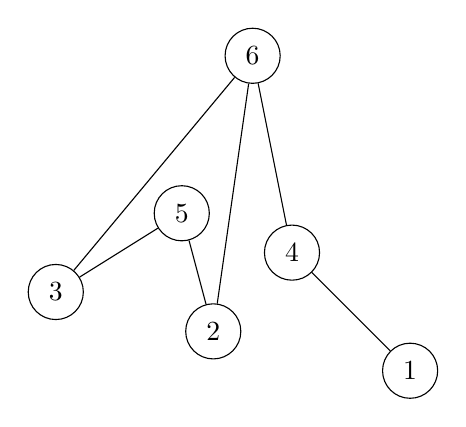
\begin{tikzpicture}[every node/.style={circle, draw, minimum size=0.7cm}]
			\node (3) at (-0.5,2) {3};
			\node (5) at (1.1,3) {5};
			\node (2) at (1.5,1.5) {2};
			\node (6) at (2,5) {6};
			\node (4) at (2.5,2.5) {4};
			\node (1) at (4,1) {1};

			\draw (3) -- (6);
			\draw (3) -- (5);
			\draw (5) -- (2);
			\draw (2) -- (6);
			\draw (1) -- (4);
			\draw (4) -- (6);
		\end{tikzpicture}
		\caption{Input graph. Already converted to be undirected and simple.}
	\end{subfigure}
	\hfill
	\begin{subfigure}[t]{0.45\linewidth}
		\centering
		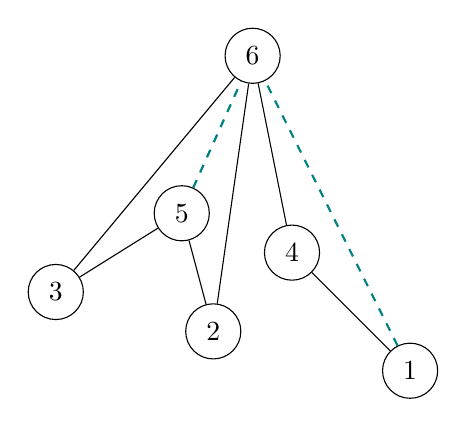
\begin{tikzpicture}[every node/.style={circle, draw, minimum size=0.7cm}]
			\node (3) at (-0.5,2) {3};
			\node (5) at (1.1,3) {5};
			\node (2) at (1.5,1.5) {2};
			\node (6) at (2,5) {6};
			\node (4) at (2.5,2.5) {4};
			\node (1) at (4,1) {1};

			\draw (3) -- (6);
			\draw (3) -- (5);
			\draw (5) -- (2);
			\draw (2) -- (6);
			\draw (1) -- (4);
			\draw (4) -- (6);

			\draw[thick, teal, dashed] (5) -- (6);
			\draw[thick, teal, dashed] (1) -- (6);
		\end{tikzpicture}
		\caption{Graph after precomputation, new shortcut edges are shown in teal.}
	\end{subfigure}
	\caption{Example of the CCH precomputation step. Nodes are named and positioned based on their rank.}
	\label{fig:cch_precomputation_example}
\end{figure}

A primary objective when selecting the vertex order is to minimize the number of shortcut edges introduced during the contraction process.
Minimizing shortcuts is beneficial for both storage and query efficiency \cite{dibbelt_customizable_2016}.
However, solely minimizing the number of added shortcuts may not be sufficient in all cases.
Different heuristics for selecting the contraction order exist.

\paragraph{Nested Dissection}

One method for computing good vertex orders are Nested Dissections.
The process begins by identifying a small, balanced separator in the graph.
Nodes within this separator are conceptually removed, partitioning the graph into smaller components.
These separator nodes are designated as high-rank nodes in the hierarchy and are consequently placed towards the end of the final node ordering.
This procedure is then applied recursively to the remaining components.
\Cref{fig:nested_dissection_example} provides a visual representation of this recursive partitioning strategy.

\begin{figure}[tbhp]
	\centering
	\begin{tikzpicture}[every node/.style={circle, draw, minimum size=1cm}]
		\node (10)                {1};
		\node (20)  [right=of 10, fill=purple!30] {3};
		\node (30)  [right=of 20] {2};
		\node (40)  [right=of 30, fill=teal!30] {21};
		\node (50)  [right=of 40] {11};
		\node (60)  [right=of 50, fill=orange!30] {18};
		\node (70)  [right=of 60] {14};

		\node (11)  [below=of 10, fill=orange!30] {9};
		\node (21)  [below=of 20, fill=orange!30] {8};
		\node (31)  [below=of 30, fill=orange!30] {7};
		\node (41)  [below=of 40, fill=teal!30] {20};
		\node (51)  [below=of 50, fill=purple!30] {12};
		\node (61)  [below=of 60, fill=orange!30] {17};
		\node (71)  [below=of 70, fill=purple!30] {15};

		\node (12)  [below=of 11] {4};
		\node (22)  [below=of 21, fill=purple!30] {6};
		\node (32)  [below=of 31] {5};
		\node (42)  [below=of 41, fill=teal!30] {19};
		\node (52)  [below=of 51] {10};
		\node (62)  [below=of 61, fill=orange!30] {16};
		\node (72)  [below=of 71] {13};

		\draw (10) -- (20) -- (30) -- (40) -- (50) -- (60) -- (70);
		\draw (11) -- (21) -- (31) -- (41) -- (51) -- (61) -- (71);
		\draw (12) -- (22) -- (32) -- (42) -- (52) -- (62) -- (72);
		\foreach \i in {1,...,7} { \draw (\i0) -- (\i1) -- (\i2); }
	\end{tikzpicture}
	\caption{Example of a Nested Dissection. The top level separator is shown in teal, the second level in orange and the third level in purple. The nodes are named according to their rank in the resulting order.}
	\label{fig:nested_dissection_example}
\end{figure}

\paragraph{Customization}

Customization assigns the current metric's weights to the original edges within the CCH supergraph \(G_C\) and initializes shortcut edge weights to infinity. Following this initialization, edge weights are systematically updated to ensure the triangle inequality holds throughout \(G_C\).

To achieve this, the concept of a lower triangle is employed.
Given an edge \(\{x, y\} \in E_C\), a lower triangle is formed by the vertices \(\{x, y, z\}\) if the edges \(\{z, x\}\) and \(\{z, y\}\) also exist, and \(rank(z) < \min\{rank(x), rank(y)\}\).
The customization algorithm iterates through the vertices of the graph in ascending order of their precomputed rank.
For each vertex \(x\), it considers all upward edges \(\{x, y\}\) in the graph, where \(y\) is a neighbor of \(x\) and \(rank(y) > rank(x)\).
For every such edge \(\{x, y\}\), we determine all lower triangles \(\{x, y, z\}\).
If the path through \(z\) offers a shorter connection, the weight of the edge \(\{x, y\}\) is updated to this smaller value: \(w(x, y) \leftarrow \min\{w(x, y), w(x, z) + w(z, y)\}\).
The detailed procedure is outlined in the pseudocode presented in \cref{alg:customization}.
An illustration of the customization process is provided in \cref{fig:cch_precomputation_example}.

Note that while the outlined algorithm only considers undirected edge weights, it can be extended to handle directed edge weights. Details can be found in \cite{dibbelt_customizable_2016}.

\begin{algorithm}
	\Input{\( G_C = (V, E_C) \), node ordering \(\pi\), edge weights \(w\)}
	\Output{Customized CCH graph}
	\BlankLine
	\ForAll{\(x\) in \(V\) in ascending order of rank}{
		\ForAll{upward edges \( \{x, y\} \) in \( E_C \)}{
			\ForAll{lower triangles \( \{x, y, z\} \) associated with \( \{x, y\} \)}{
				\( w(x, y) \longleftarrow \min\{ w(x, y), w(x, z) + w(z, y) \} \)\;
			}
		}
	}
	\caption{CCH Customization}
	\label{alg:customization}
\end{algorithm}

\begin{figure}[tbhp]
	\begin{subfigure}[t]{0.45\linewidth}
		\centering
		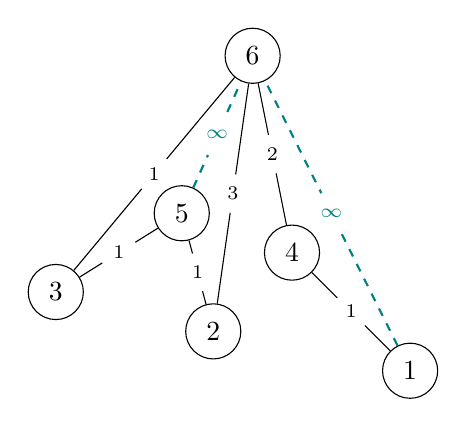
\begin{tikzpicture}
			\begin{scope}[every node/.style={circle, draw, minimum size=0.7cm}]
				\node (3) at (-0.5,2) {3};
				\node (5) at (1.1,3) {5};
				\node (2) at (1.5,1.5) {2};
				\node (6) at (2,5) {6};
				\node (4) at (2.5,2.5) {4};
				\node (1) at (4,1) {1};
			\end{scope}

			\begin{scope}[every node/.style={midway, fill=white, font=\scriptsize, inner sep=1mm, circle}]
				\draw (3) -- (6) node {1};
				\draw (3) -- (5) node {1};
				\draw (2) -- (5) node {1};
				\draw (2) -- (6) node {3};
				\draw (1) -- (4) node {1};
				\draw (4) -- (6) node {2};
				\draw[thick, teal, dashed] (5) -- (6) node {\(\infty\)};
				\draw[thick, teal, dashed] (1) -- (6) node {\(\infty\)};
			\end{scope}
		\end{tikzpicture}
		\caption{Graph after precomputation. Weights are added to the edges. Shortcuts get weight \(\infty\).}
	\end{subfigure}
	\hfill
	\begin{subfigure}[t]{0.45\linewidth}
		\centering
		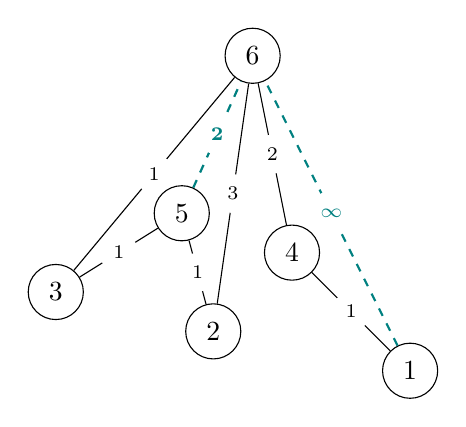
\begin{tikzpicture}
			\begin{scope}[every node/.style={circle, draw, minimum size=0.7cm}]
				\node (3) at (-0.5,2) {3};
				\node (5) at (1.1,3) {5};
				\node (2) at (1.5,1.5) {2};
				\node (6) at (2,5) {6};
				\node (4) at (2.5,2.5) {4};
				\node (1) at (4,1) {1};
			\end{scope}

			\begin{scope}[every node/.style={midway, fill=white, font=\scriptsize, inner sep=1mm, circle}]
				\draw (3) -- (6) node {1};
				\draw (3) -- (5) node {1};
				\draw (2) -- (5) node {1};
				\draw (2) -- (6) node {3};
				\draw (1) -- (4) node {1};
				\draw (4) -- (6) node {2};
				\draw[thick, teal, dashed] (5) -- (6) node {\textbf{2}};
				\draw[thick, teal, dashed] (1) -- (6) node {\(\infty\)};
			\end{scope}
		\end{tikzpicture}
		\caption{Graph after customization. The shortcut edge \(\{5, 6\}\) is updated to weight \(2\).}
	\end{subfigure}
	\caption{Example of the CCH customization step.}
\end{figure}

\paragraph{Query}

To answer a shortest path query between a source node \(s\) and a target node \(t\), the algorithm utilizes an structure known as the elimination tree.
The elimination tree is defined on the nodes of \(G_C\).
The parent of a node \(v\) in the elimination tree is the neighbor \(p\) of \(v\) in the CCH graph that has the lowest rank among all neighbors with a rank strictly greater than the rank of \(v\).
\cref{fig:cch_elimination_tree} illustrates the elimination tree for the example graph shown in \cref{fig:cch_precomputation_example}.
The query algorithm performs a bidirectional search upwards in this elimination tree, starting from \(s\) and \(t\).

\begin{figure}[tbhp]
	\centering
	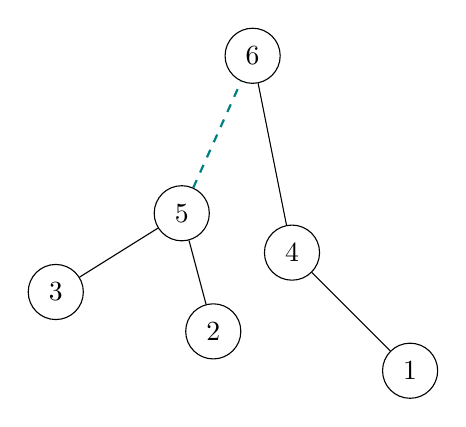
\begin{tikzpicture}[every node/.style={circle, draw, minimum size=0.7cm}]
		\node (3) at (-0.5,2) {3};
		\node (5) at (1.1,3) {5};
		\node (2) at (1.5,1.5) {2};
		\node (6) at (2,5) {6};
		\node (4) at (2.5,2.5) {4};
		\node (1) at (4,1) {1};

		\draw (3) -- (5);
		\draw (5) -- (2);
		\draw (1) -- (4);
		\draw (4) -- (6);

		\draw[thick, teal, dashed] (5) -- (6);
	\end{tikzpicture}
	\caption{Elimination tree for the example graph in \cref{fig:cch_precomputation_example}.}
	\label{fig:cch_elimination_tree}
\end{figure}

The core query process operates iteratively.
Let \(u_s\) and \(u_t\) be the current nodes in the upward search originating from \(s\) and \(t\), respectively; initially, \(u_s = s\) and \(u_t = t\).
The algorithm proceeds until the root of the elimination tree is reached.
In each step, the ranks of the current nodes \(u_s\) and \(u_t\) are compared.
If \(u_s\) has a smaller rank than \(u_t\), the algorithm relaxes all outgoing edges \(\{u_s, v_i\}\) present in \(G_C\).
Subsequently, \(u_s\) is updated to become its parent node in the elimination tree.
Otherwise (if \(u_t\) has a rank less than or equal to that of \(u_s\)), the algorithm relaxes all outgoing edges \(\{u_t, v_i\}\) existing in the CCH graph.
Following the relaxation step, \(u_t\) is updated to its parent in the elimination tree.
This process continues, effectively exploring paths upwards towards higher-ranked nodes.
The correctness of this query algorithm for computing shortest path distances has been established; a detailed proof, which is beyond the scope of this thesis, can be found in \cite{dibbelt_customizable_2016}.

\paragraph{Complexity}

The size of the separators found significantly impacts the efficiency of CCH queries.
CCH queries restrict exploration to edges leading towards higher-ranked nodes (upward edges).
Consider the separator identified at the highest level of the recursion, which contains approximately \(n^\beta\) nodes.
When a query initiates within a component defined by this separator, nodes located in other components cannot be reached without traversing downwards through a separator node, violating the upward search constraint.
This containment effect applies recursively within the sub-components generated during the nested dissection.
Let \(\alpha\) denote the balance factor.
The sub-components at recursion level \(i\) consequently have a size of at most \( \alpha^i \cdot n \).
Analyzing the total bound of the search space involves summing these separator sizes across the finite levels \(i\) of the recursion.
This sum can be bounded by approximating it with the corresponding infinite geometric series \cite{bauer_search-space_2016}:

\begin{align*}
	    & ~\sum_{i=0}^{\infty} (\alpha^i\cdot n)^\beta                                                         \\
	=   & ~n^\beta \cdot \sum_{i=0}^{\infty} \alpha^{i\cdot \beta}                                             \\
	=   & ~n^\beta \cdot \frac{1}{1 - \alpha^\beta} \qquad \text{Geometric series, since \(\alpha \in (0,1)\)} \\
	\in & ~\bigO{n^\beta}
\end{align*}

This analysis demonstrates that the total search space size explored during a CCH query is bounded by \(\bigO{n^\beta}\), under the assumption that small separators can be found recursively.
Note that while we do not have worst-case guarantees for the separator sizes in real road networks, they are expected to be small in practice.
Thus, the performance of the CCH algorithm is directly linked to the ability to find small separators.
